\documentclass[a4paper]{article}

\usepackage[english]{babel}
\usepackage[utf8]{inputenc}
\usepackage{amsmath}
\usepackage{listings}
\usepackage{color}
\usepackage{hyperref}
\usepackage{float}
\usepackage{graphicx}
\graphicspath{{../pics/}}

\title{Machine Learning (course 1DT071)
Uppsala University – Spring 2015
Report for Assignment 3 by group 2}

\author{Ludvig Sundstr\"{o}m and John Shaw}
\date{\today}

\begin{document}

\maketitle

\section*{Task 1: Training on simple 3-dimensional data}

\subsection*{Question 1} 

\emph{Use } \texttt{plotsomehits} \emph{ to study the overlap between the winning nodes for the two clusters, as above. What amount of overlap do you see for each different data set?}

\textbf{Answer:} As the sparseness increases, we expect the amount of overlap between the clusters to increase as well. We confirmed this by plotting the winning nodes from the map trained on the P10 dataset as well as the nodes from map trained on the P30 dataset. The winning nodes from the map trained on the more dense data were much closer together than the nodes trained on the P30 dataset. 

\subsection*{Question 2}
\emph{Explain why the two }\texttt{plotsomhits} \emph{ figures that you created for Plot 1 look the way they do.}

\textbf{Answer:} Figure \ref{fig:q1_somP10onP30} displays the winning nodes of the SOM trained on the most dense data applied on the most sparse data. Since the data is much more sparse than the distribution of nodes, the nodes on the edge of the map is most likely to win. Figure \ref{fig:q1_somP30onP10} displays the winning nodes of the SOM trained on the most sparse data applied on the most dense data. Here, a couple nodes inside the map close to the dense cluster are most likely to win. 

\begin{figure}[H] %float here
	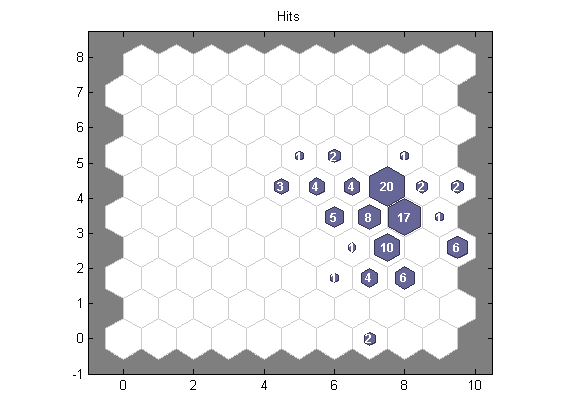
\includegraphics[scale=0.7]{q1_somP30onP10.png}
	\caption{\label{fig:q1_somP30onP10}\textbf{Plot 1} Picture of cluster $F_1$ when using SOM\_P30 on P10.}
\end{figure}
\begin{figure}[H] %float here
	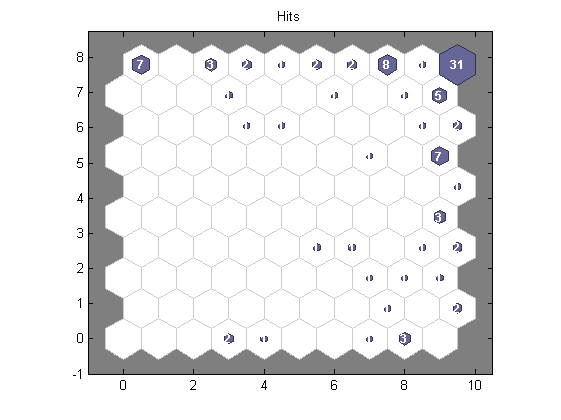
\includegraphics[scale=0.7]{q1_somP10onP30.png}
	\caption{\label{fig:q1_somP10onP30}\textbf{Plot 1} Picture of cluster $F_1$ when using SOM\_P10 on P30.}
\end{figure}

\section*{Task 2: Mapping of RGB color data}

\subsection*{Question 3}
\emph{What relation between the ordering phase and tuning phase seems to be best in order to get a smooth map? Why do you think that is?}

\textbf{Answer:} 
In this problem, the data lies in 3-dimensional space. In order to make the map cover the data in the best way possible, we try to visualize the problem. Since the map is 2-Dimensional and the target data 3-Dimensional, we think of the map as a paper arc which is formed in some way to occupy as much space as possible in a cube with data points evenly distributed in it. In this problem it is more important to have smooth transitions between nodes than to have a full variation of all the colors. Therefore, we want the map to take a smooth shape eventually in order to to minimize the difference of the distances between the nodes. To train a map in such a way, we found that we needed to train the network with no tuning phase at all. If we added a tuning phase where the nodes are moved individually, the distances start to differ and the shape of the map was distorted, resulting in a non-smooth color plot. The network had 10$\cdot$10 nodes, an initial neighbourhood size of 5 and was trained for 500 epochs. The result of this training is seen in figure \ref{fig:plot1P10onP30}.

\begin{figure}[H] %float here
	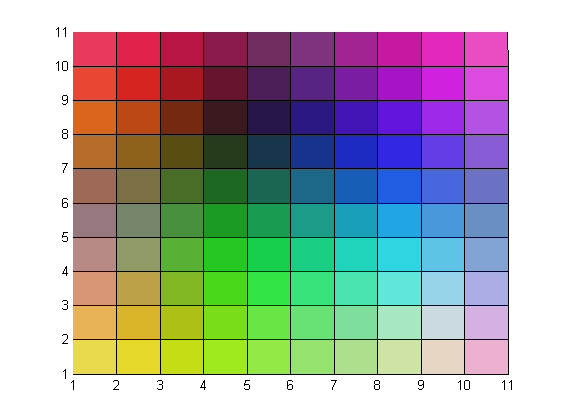
\includegraphics[scale=0.7]{q2_Order500_15init_500epoch.png}
	\caption{\label{fig:plot1P10onP30}\textbf{Plot 2} Picture of a good gradient. 500 epochs ordering phase with an initial neighbourhood size of 5 nodes.}
\end{figure}
\pagebreak
\section*{Task 3: Analysis on wine data}

\subsection*{Question 4}
\emph{What training parameters did you use? How well does the trained
SOFM separate the classes in your opinion? Is some class easier to separate then the rest? If so, which one?}

\textbf{Answer:} We obtained the best results when we trained the map for 200 epochs in total with only one epoch in ordering phase. The first class was easier to separate from the others, but we found this data difficult to train on and the algorithm performed quite badly.

\subsection*{Question 5}
\emph{What training parameters did you use? What  major differences
do you see in the results compared to the 5 by 5-node SOFM?}

\textbf{Answer:} This time we used a 10 times 10 network and the same parameters except that we trained for 300 epochs instead of 200 epochs. We managed to get better precision in the classification, probably since the previous number of 25 nodes was not enough to cover the training data. With 100 nodes we get better coverage over both the sparse cluster and the two more dense clusters. Even though they were overlapping a bit the new map was able to cover that area and separate them better than the $5\cdot5$ map. 


\subsection*{Question 6}
\emph{How well do the SOFM separate the classes in the normalized
data?}

\textbf{Answer:} Normalizing the data greatly improved the quality of the classification. We achieved without difficulties three very clear groups of winning nodes representing the different wine types. In this problem, we are interested in identifying three clusters. Again, it's not that important to cover all data, in fact if there are data points that differ much from the rest they might distort the data. So this is obviously an example of a problem where you benefit from normalizing the data. 

\pagebreak
\section*{Task 4: Analysis of flower data}

%\subsection*{Question 7}
%\emph{How well does the SOFM separate the classes, in your opinion?}
 
 %\textbf{Answer: } When studying the sample hit plots it clearly shows that there are a minimum of two classes since two of them are clustered in opposite sides (namely \ref{fig:plotg1} and \ref{fig:plotg3}). However it's hard to tell if the cluster in the middle \ref{fig:plotg2} is actually another class even if we could suspect this without known anything about the data.

%TODO In this classification problem, the map clearly distinguishes a distance between two groups of nodes. It does not however clearly classify the three flower classes. One possible reason is that the characteristics of one class of Iris flowers are very similar to another class characteristics making it hard for a SOFM to classify. 

\subsection*{Question 7 / 8}
\emph{How well did the SOM separate the classes and if you did not already know that the data came from three different species of Iris flowers, could you have found any evidence in the neighbour distances plot to indicate that the data are not from a single species? What evidence would that be, and what does it imply about the distribution of the data?
Describe your reasoning.}

 \textbf{Answer: } As with the wine-data the goal of this section was to attempt to train a SOM classify three different types of data, this time Iris flowers. We didn't manage to train a map on this data with the same success as with the wine data but we made some interesting observations anyways. \\ By studying the neighbourhood distance plot, we see a clear distance between two groups of nodes. It is possible that the smaller part could represent one type of flower. To investigate further, we plot the winning nodes of the three individual groups of data. Although we see some overlapping between the different groups, we can still see a clear partition of the map according to the three groups. Judging from this, the first samples are from a species which differs quite much from the others, while the data from the other two species probably are very close as two clusters but still possible to separate. (There might be some data points for which it is possible that to origin from different species).

  \begin{figure}[H] %float here
	 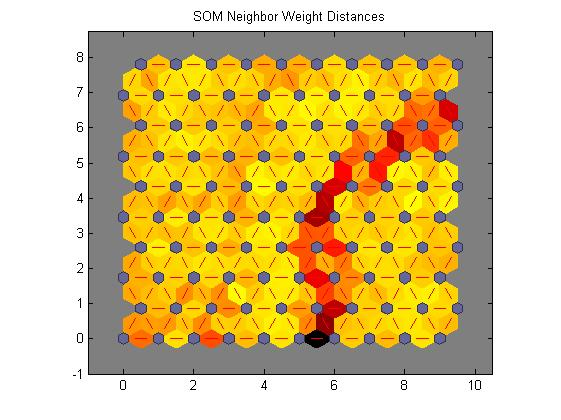
\includegraphics[scale=0.5]{q4_100o_1900tuningphase.jpg}
	 \caption{\label{fig:neighbour} Neighbourhood distance for the flower data.}
 \end{figure}
 \begin{figure}[H] %float here
	 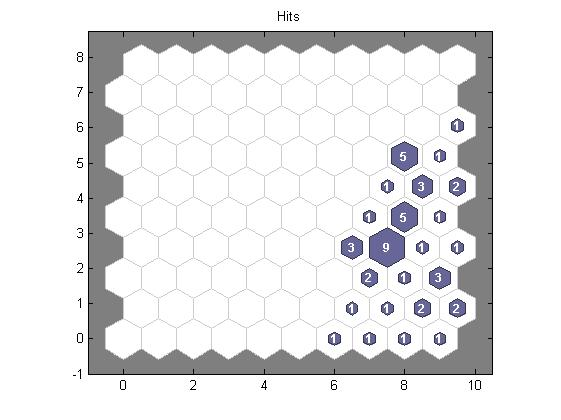
\includegraphics[scale=0.5]{q4_plotsom1_50.jpg}
	 \caption{\label{fig:plotg1} Analysis of flower data, the first group.}
 \end{figure}
  \begin{figure}[H] %float here
	 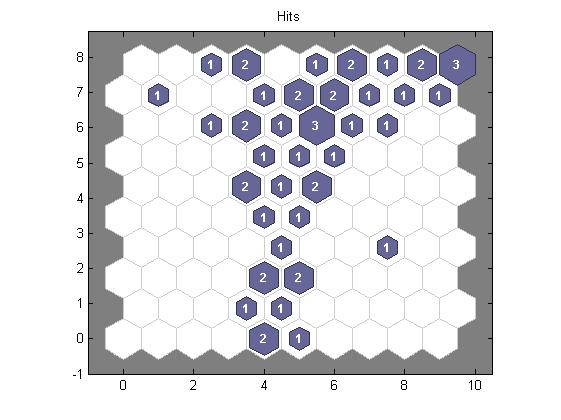
\includegraphics[scale=0.5]{q4_plotsom50_100.jpg}
	 \caption{\label{fig:plotg2} Analysis of flower data, the second group.}
 \end{figure}
  \begin{figure}[H] %float here
	 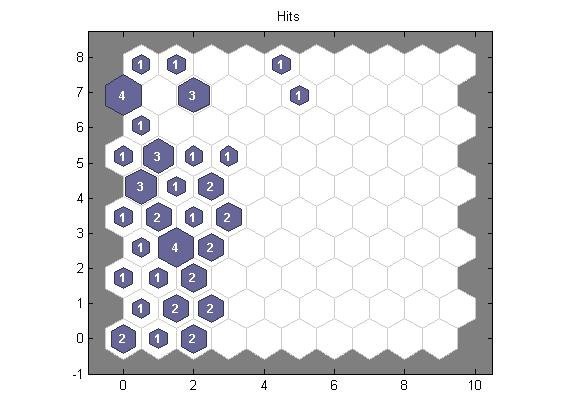
\includegraphics[scale=0.5]{q4_plotsom100_150.jpg}
	 \caption{\label{fig:plotg3} Analysis of flower data, the third group.}
 \end{figure}
%\textbf{Answer:} We can clearly see that there are two classes when analysing the neighbourhood distances since there are a clear line dividing the classes in two \ref{fig:neighbour}. However the third class is not visible. We tried to train SOM networks to classify the datasets 1vs1 as well and clearly it can't separate two of the sets. This suggest that two of the sets are very hard to separate with the SOM and this setup. 

%We were discussing this findings with Peter Backeman and we found out that Matlab actually doesn't specify the colour coding of the regions so without being able to access the weights directly we can't speculate much more about them. 


%The neighbor distances plot tells us that a certain set of data differs alot from another set of data. This implies that the data is probably not entirely from the same class of flowers. In this case it is difficult to interperet three classes from the generated SOFM, probably because of two data clusters overlapping. 

\subsection*{Question 9}
\emph{Do any of the attributes seem particularly correlated? Which
ones? Explain your reasoning.}

\textbf{Answer:}  We can see in the SOM input planes that the petal length and the petal width is very correlated. Both classes have black areas in the same region and the main difference seem to be the yellow region (This are refereed to as input 3 and 4 in \ref{fig:weightdist}). 

\subsection*{Question 10}
\emph{Which species has the smallest petals? Which species has the
largest petals? Explain your reasoning.}

\textbf{Answer:} 
In figure \ref{fig:weightdist}, dark colors indicate weak connections and light colors shows the strongest positive connections. Further looking at the input planes 3 and 4, we see that the group representing the left part of both input map 3 and 4 area has the most positive connections and hence the largest petals, and in a similar way the area representing the right part of the map has the smallest petals. Referencing to figure \ref{fig:plotg1} and \ref{fig:plotg3} we see establish group 3(Iris Virganica) to have the largest petals and group 1 (Iris Setosa) to have the smallest petals.

  \begin{figure}[H] %float here
	 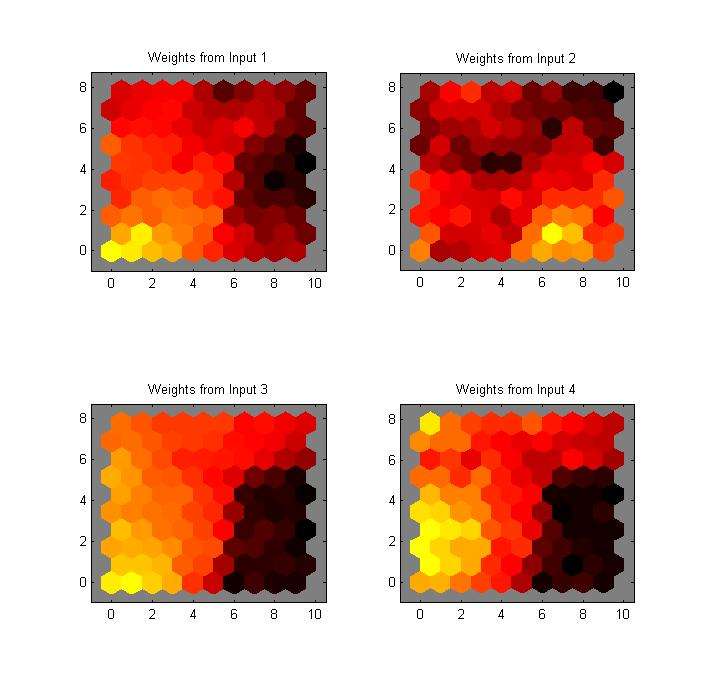
\includegraphics[scale=0.45]{q4_q9weightdistribution.jpg}
	 \caption{\label{fig:weightdist} Weight distribution for flower data.}
 \end{figure}
\section*{Task 5: Analysis of unknown data}


\subsection*{Question 11}
\emph{How many well-separated clusters are there in the data set?
Explain how you found out your answer. Include figures if necessary.}


 \textbf{Answer:} By studying the neighbour distances shown in figure \ref{fig:20x20trainedUnknown} and we identify 7 separated clusters. However, since the SOFM creates a 2-dimensional map that tries to fit in a 10-dimensional space, some of these areas in 2-dimensions might be connected to each other at the borders of the network. We strongly suspect that the bottom left one and the top left one are connected since the lines of the separation fits very good with each other. This means it's only 5 different actual clusters. If we imagine the 2D neural network as a paper it have connected two corners on one side and created a loop where the edges are against each other. 
 
We found the best results with 200 epochs and no tuning phase. We used a $20 \times 20$ sized network.

 \begin{figure}[H] %float here
	 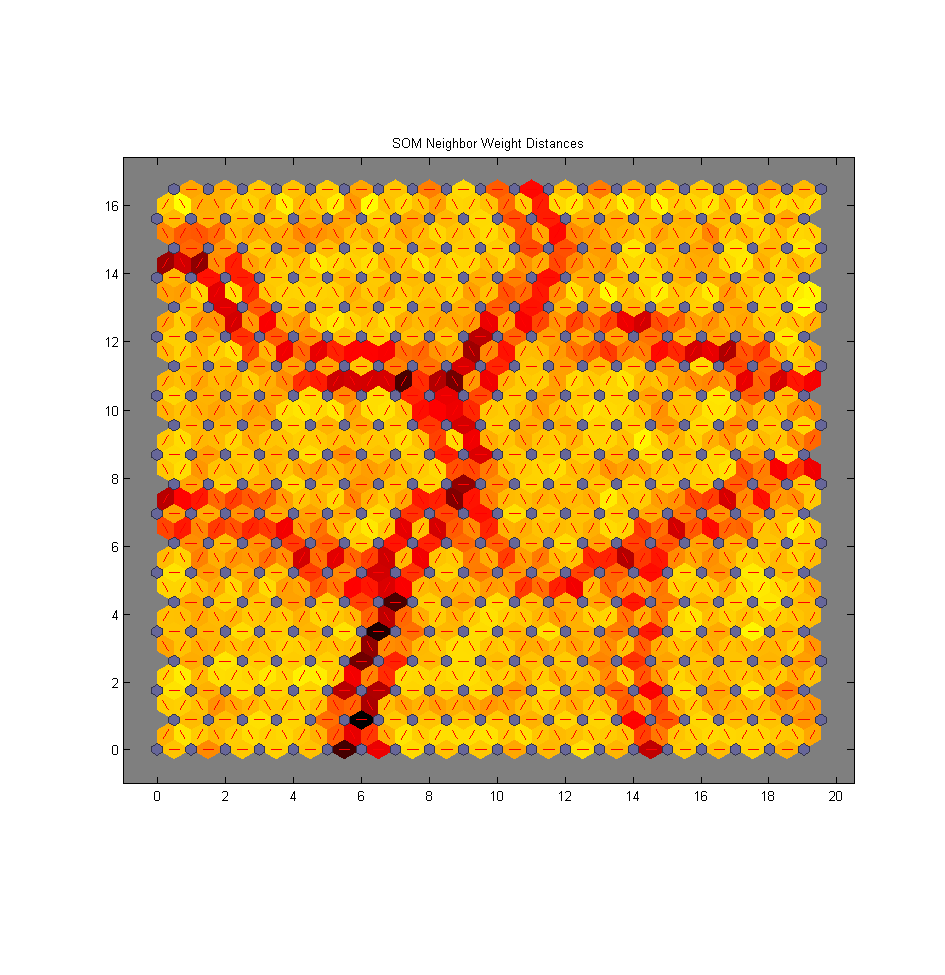
\includegraphics[scale=0.4]{20x20trainedUnknown.png}
	 \caption{\label{fig:20x20trainedUnknown} Picture showing the neighbourhood of the nodes in a SOM trained for the unknown data.}
 \end{figure}

\subsection*{Question 12}
\emph{Which data points are from the same cluster? How did you
figure it out? Include figures if necessary.} 

\textbf{Answer:} We used the \texttt{plotsomhits} with the trained SOM and the points as input parameters. If we compare their location we can see that point 1 and 4 are close to each other. Point 3 and 5 are very close to each other as well but are far away from 1 and 4. Point 2 is placed in the top left corner so it could belong to a separated cluster or possible to the same class as 3 and 5 the bottom left corner.

 \begin{figure}[H] %float here
	 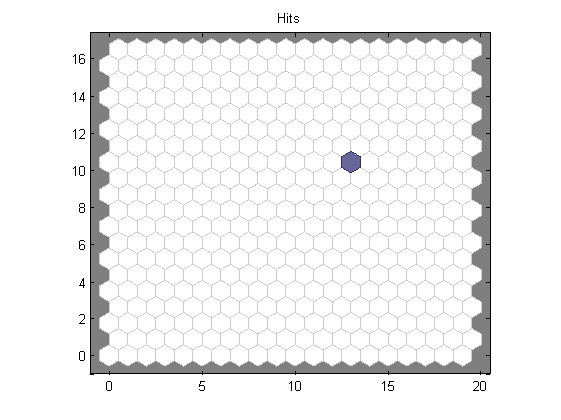
\includegraphics[scale=0.5]{point1.png}
	 \caption{\label{fig:point1} Weight triggered by point 1 in our trained SOM.}
 \end{figure}
 \begin{figure}[H] %float here
	 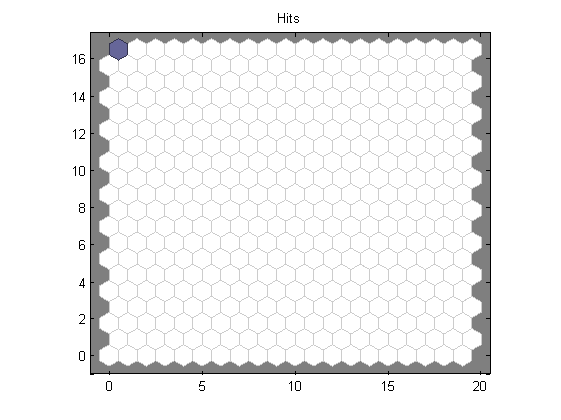
\includegraphics[scale=0.5]{point2.png}
	 \caption{\label{fig:point2} Weight triggered by point 2 in our trained SOM.}
 \end{figure}
 \begin{figure}[H] %float here
	 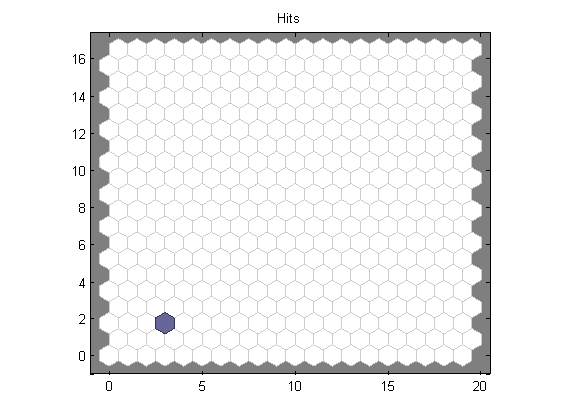
\includegraphics[scale=0.5]{point3.png}
	 \caption{\label{fig:point3} Weight triggered by point 3 in our trained SOM.}
 \end{figure}
 \begin{figure}[H] %float here
	 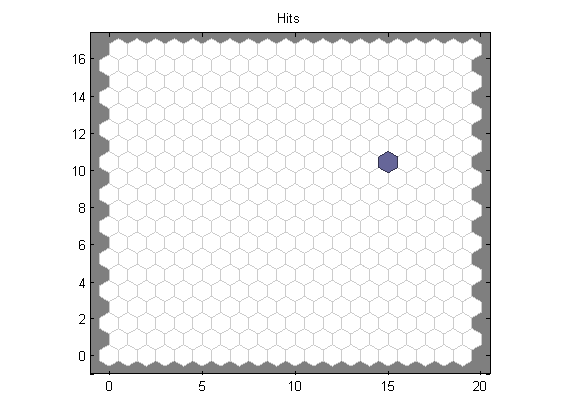
\includegraphics[scale=0.5]{point4.png}
	 \caption{\label{fig:point4} Weight triggered by point 4 in our trained SOM.}
 \end{figure}
 \begin{figure}[H] %float here
	 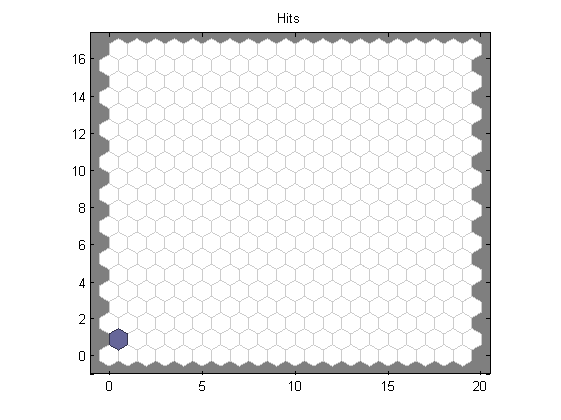
\includegraphics[scale=0.5]{point5.png}
	 \caption{\label{fig:point5} Weight triggered by point 5 in our trained SOM.}
 \end{figure}
 \pagebreak
\section*{Task 6: Wrapping up}

\subsection*{Question 13}
\emph{Propose a real-world problem that you consider interesting and
that you believe can be solved using a SOFM. Explain in a few sentences how the
SOFM would be used, and what kind of data that it would be trained on.}

\textbf{Answer:} SOFM can be used to train a recommendation engine for a web-shop. The data it can be used for training is sets of what customers have bought earlier and then it should be able to find out if additional things are more likely to be appealing for a customer who is interested in a certain thing. 
A similar SOFM can help deciding what type of things should be exposed together in a store. 
If we have large amount of audio samples we can try to classify what the conversations are about. This can be useful for on-line phone conversation analysis to detect terrorism or teens planning to download illegal movies. 
\end{document}
